\documentclass[a4paper,10pt]{article}
%\documentclass[a4paper,10pt]{scrartcl}
\usepackage[ngerman]{babel}
\usepackage[utf8]{inputenc}

\title{Kartendarstellungen mit\\matplotlib Toolkit basemap}
\author{Simon von Hall}
\date{}

\pdfinfo{%
  /Title    (Kartendarstellungen)
  /Author   (Simon von Hall)
  /Creator  ()
  /Producer ()
  /Subject  ()
  /Keywords ()
}

\begin{document}
\maketitle
\clearpage
\tableofcontents
\section{Motivation}
\label{sec:1}
\section{Kartendarstellungen}
\label{sec:2}
 \subsection{Azimuthale äquidistante Projektion}
\label{sec:azimuequi}
Bei dieser Projektion ist die kürzeste Entfernung vom Mittelpunkt der Karte zu einem beliebigen anderen Punkt eine gerade Linie. Das bedeutet, dass alle Punkte, die auf einem Kreis um den Kartenmittelpunkt liegen, äquidistant sind.\\
Nachteil:\newline
Die Gebiete die auf der anderen Seite der Welt liegen, werden sehr verzehrt dargestellt. Daher ist diese Projektion für Weltkarten 
eher ungeeignet.\\
\begin{figure}[hbtp]
\centering
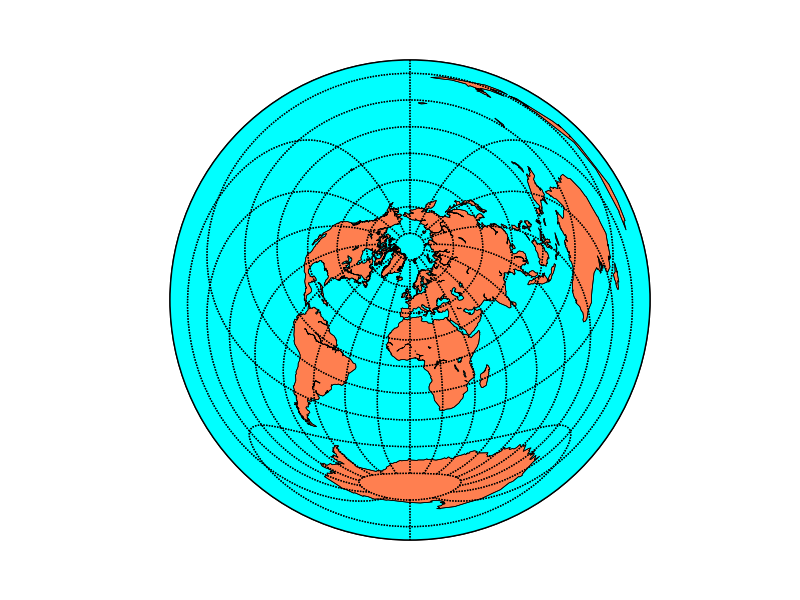
\includegraphics[scale=0.4,origin=c]{/Users/student/seminar/Kartendarstellungen/seminar/aziequi} \\
\caption{Azimuthale äquidistante Projektion}
\end{figure}
\clearpage
\subsection{Gnomonische Projektion}
\label{sec:gnomic}
In der gnomonischen Projektion werden alle Längenkreise als gerade Linien dargestellt.
Das Besondere der gnomonischen Projektion ist das der Projektionspunkt im Mittelpunkt der Erde liegt.
Da hier von Innen nach Außen projiziert wird, nimmt die Verzerrung mit der Entfernung vom Kartenmittelpunkt zu. Die gnomonische Projektion ist keine globale Projektion.\\

\begin{figure}[hbtp]
\centering
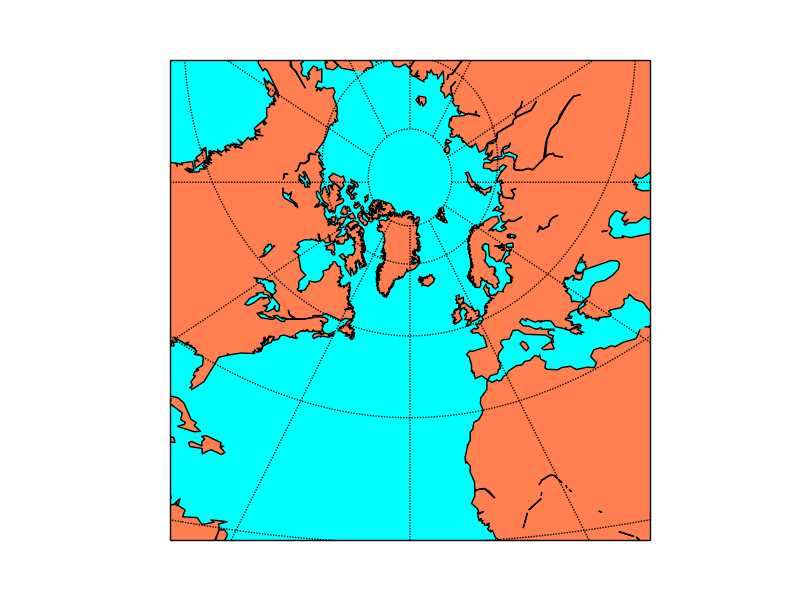
\includegraphics[scale=0.5,origin=c]{/Users/student/seminar/Kartendarstellungen/seminar/gnom} \caption{Gnomonische Projektion}
\end{figure}
\newpage 
\subsection{Orthographic Projection}
\label{sec:2.3}

\subsection{Geostationäre Projektion}
\label{sec:geostat}
In der geostationären Projektion wird die Erde aus der Perspektive eines geostationären Satelliten.
Vorteil:\newline \begin{itemize}
                  \item Wenn die Position des Satelliten bekannt ist, kann man dessen
                  Bilder als Hintergrund verwenden (siehe \ref{bilder})
                 \end{itemize}

Nachteil:\newline \begin{itemize}
                  \item Die andere Seite der Erde wird nicht dargestellt.\\
                  \item Entfernungen zwischen 2 Punkten werden auf Kreisbögen gemessen.\\
                  \item Der Satellit muss über dem Äquator sein.
                 \end{itemize}
\begin{figure}[hbtp]
\centering
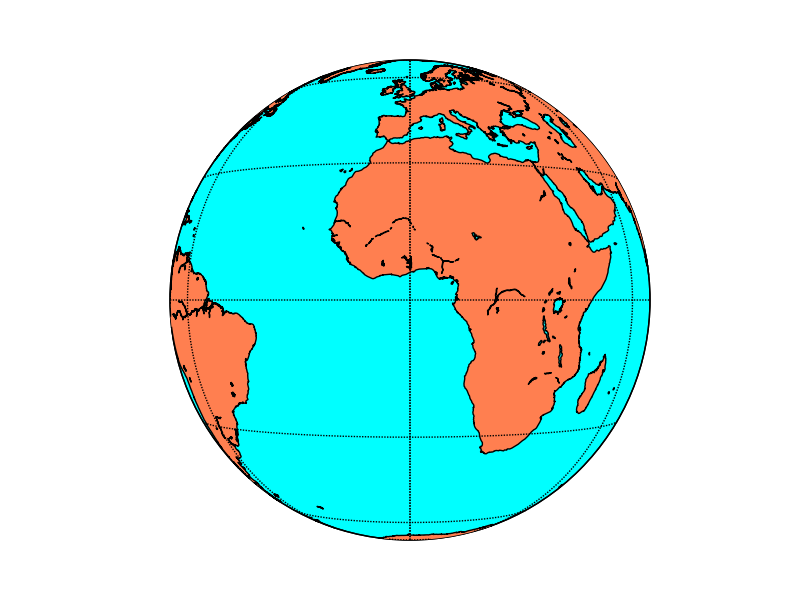
\includegraphics[scale=0.5,origin=c]{/Users/student/seminar/Kartendarstellungen/seminar/geos} \caption{Geostationäre Projektion}
\end{figure}
\newpage 
\subsection{Near-Sided perspektivische Projektion}
\label{sec:nearsideperspective}
Die Near Sided Perspective zeigt die Erde aus der Sicht eines Satelliten. Also ist es im Prinzip das selbe
wie die geostationäre Projektion.
\subsection{Mollweide Projection}
\label{sec:Mollweiden}
Bei der Mollweiden Projektion wird die Erde als Oval dargestellt. Die Mollweiden Projektion ist flächentreu.
Der Äquator und der Nullmeridian werden bei der Mollweiden Projektion maßstabsgetreu wieder gegeben.
Breitenkreise werden bei der Mollweiden Projektion als Geraden dargestellt. Die Längenkreise sind als Ellipsen dargestellt.
\subsection{Hammer Projektion}
\label{sec:Hammer}
Die Hammer Projektion ist wie die Mollweiden Projektion eine flächentreue Projektion.
Bei der Hammer Projektion wird die Erden ebenfalls als Oval dargestellt. Allerdings werden die Breitenkreise im Gegensatz zur Mollweiden Projektion als Ellipsen dargestellt, dadurch ist die Verzerrung an den Rändern nicht so stark. Nachteil bei dieser Art der Darstellung ist, dass die Erde an den Polen gestaucht wird.
\subsection{Robinson Projection}
\label{sec:2.8}
\subsection{Eckert IV Projection}
\label{sec:2.9}
\subsection{Kavrayskiy VII Projection}
\label{sec:2.10}
\subsection{McBryde-Thomas Flat Polar Quartic}
\label{sec:2.11}
\subsection{Sinusoidal Projection}
\label{sec:2.12}
\subsection{Equidistant Cylindrical Projection}
\label{sec:2.13}
\subsection{Cassini Projection}
\label{sec:2.14}
\subsection{Mercator Projection}
\label{sec:2.15}
\subsection{Transverse Mercator Projection}
\label{sec:2.16}
\subsection{Oblique Mercator Projection}
\label{sec:2.17}
\subsection{Polyconic Projection}
\label{sec:2.18}
\subsection{Miller Cylindrical Projection}
\label{sec:2.19}
\subsection{Gall Stereographic Projection}
\label{sec:2.20}
\subsection{Cylindrial Equal-Area Projection}
\label{sec:2.21}
\subsection{Lambert Conformal Projection}
\label{sec:2.22}
\subsection{Lambert Azimuthal Equal Area Projection}
\label{sec:2.23}
\subsection{Stereographic Projection}
\label{sec:2.24}
\subsection{Equidistant Conic Projection}
\label{sec:2.25}
\subsection{Albers Equal Area Projection}
\label{sec:2.26}
\subsection{Polar Stereographic Projection}
\label{sec:2.27}
\subsection{Polar Lambert Azimuthal Projection}
\label{sec:2.28}
\subsection{Polar Azimuthal Equidistant Projection}
\label{sec:2.29}
\subsection{van der Grinten Projection}
\label{sec:2.30}
\section{Erstellen von Karten mit basemape}
\label{sec:3}

\end{document}
